\chapter{Конструкторский раздел}

В данном разделе будут спроектированы схемы алгоритмов, произведена оценка трудоемкости алгоритмов, описаны используемые типы данных, а также произведена оценка памяти и описана структура ПО.

\section{Схемы алгоритмов}

В следующих схемах массив будет представлен как $A$, $N$ - размер массива, а $A_{i}$ - i-ый элемент массива.

На рисунках 2.1 - 2.3 представлены схемы рассматриваемых алгоритмов.
 
\newpage
\begin{figure}[h!]
	\begin{center}
		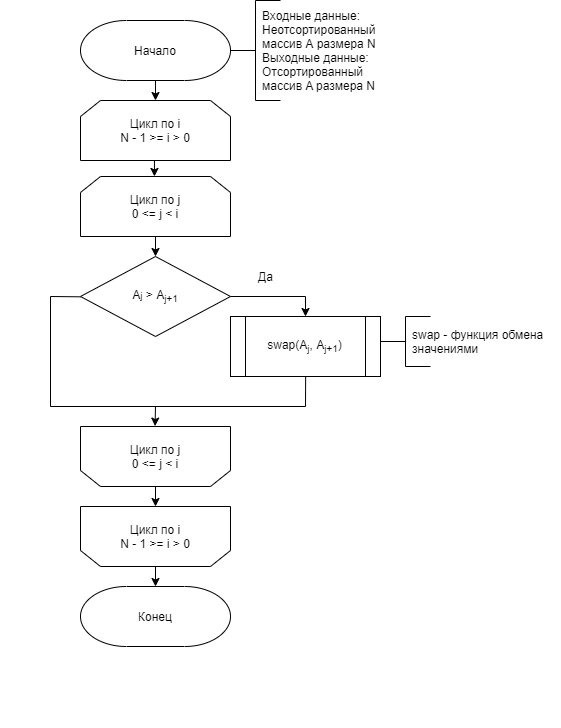
\includegraphics[scale=0.6]{assets/bubbleSort.png}
	\end{center}
	\caption{Схема алгоритма сортировки пузырьком}
\end{figure}

\newpage 
\begin{figure}[h!]
	\begin{center}
		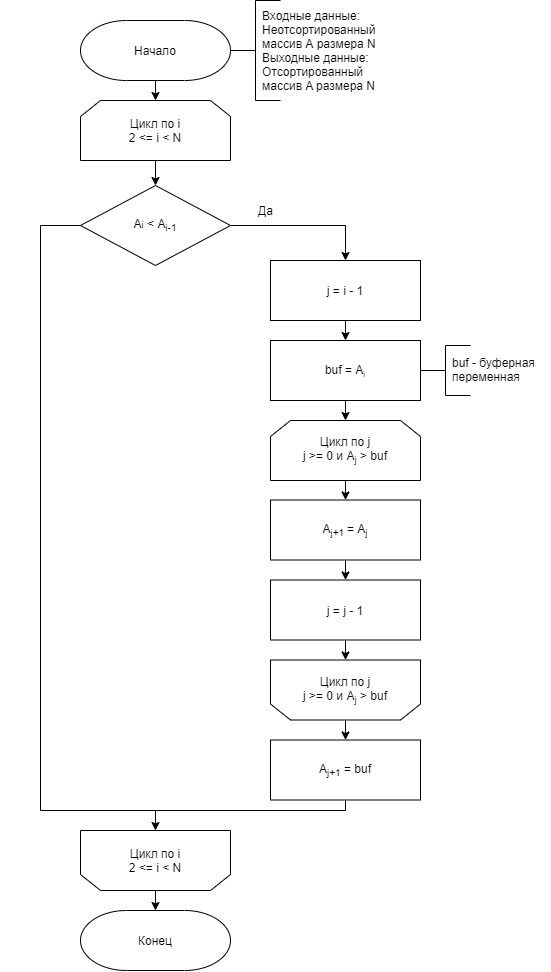
\includegraphics[scale=0.6]{assets/insertionSort.png}
	\end{center}
	\caption{Схема алгоритма сортировки вставками}
\end{figure}

\newpage 
\begin{figure}[h!]
	\begin{center}
		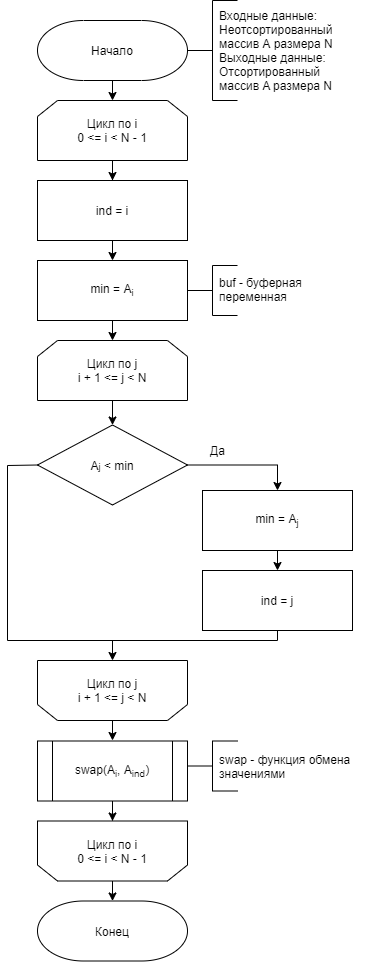
\includegraphics[scale=0.6]{assets/selectionSort.png}
	\end{center}
	\caption{Схема алгоритма сортировки выбором}
\end{figure}

\newpage
\section{Модель оценки трудоемкости алгоритмов}

\subsection{Трудоемкость алгоритмов}

Введем модель оценки трудоемкости.

\begin{enumerate}
	\item Трудоемкость базовых операций
		\begin{itemize}
			\item Примем трудоемкость следующих операций равной 1:
			\begin{equation}
				=, +, -, +=, -=, ==, !=, <, >, \leq, \geq, !, \&\&, ||, []
			\end{equation}
			\item Примем трудоемкость следующих операций равной 2:
			\begin{equation}
				*, /, \%, *=, /=,
			\end{equation}
		\end{itemize}
	\item Трудоемкость циклов
	\begin{equation}
		f = f_{init} + f_{compare} + N_{iter} * (f_{body} + f_{inc} + f_{compare})
	\end{equation}
	\item Трудоемкость условного оператора
		Пусть трудоемкость самого условного перехода равна 0. Тогда
		\begin{equation}
			f_{if} = f_{condition} + 
			\begin{sqcases}
				min(f_{true}, f_{false}), \text{в лучшем случае}\\
				max(f_{true}, f_{false}), \text{в худшем случае}\\				
			\end{sqcases}
		\end{equation}
\end{enumerate}

где \newline
$f_{init}$ - трудоемкость инициализации, \newline
$f_{compare}$ - трудоемкость сравнения, \newline
$N_{iter}$ - количество итераций, \newline
$f_{body}$ - трудоемкость тела цикла, \newline
$f_{inc}$ - трудоемкость инкрементации, \newline
$f_{condition}$ - трудоемкость условия, \newline
$f_{true}$, $f_{false}$ - трудоемкость веток условного оператора.
\newpage

\subsection{Трудоемкость сортировки выбором}

Трудоемкость для сортировки выбором состоит из:
\begin{itemize}
	\item Трудоемкость внешнего цикла:
	\begin{equation}
		f_{outer} = 3 + 13(N - 1)
	\end{equation}		
	\item Суммарная трудоемкость внутренних циклов при повторах [1..N - 1]:
	\begin{equation}
		f_{inner} = 2(N - 1) + \frac{N(N - 1)}{2} \cdot f_{if}
	\end{equation}
	\item Трудоемкость условия внутреннего цикла:
	\begin{equation}
		f_{if} = 2 + \begin{sqcases}
						0, & \text{л.с.}\\
						3, & \text{х.с.}\\
					 \end{sqcases}
	\end{equation}
\end{itemize}

Тогда в лучшем случае трудоемкость будет равна

\begin{equation}
	f = -12 + 14N + N^2 \approx N^2 = O(N^2)
\end{equation}

В худшем случае

\begin{equation}
	f = -12 + 12.5N + \frac{5}{2}N^2 \approx N^2 = O(N^2)
\end{equation}

\subsection{Трудоемкость сортировки вставками}

Трудоемкость для сортировки вставками состоит из:
\begin{itemize}
	\item Трудоемкость внешнего цикла:
	\begin{equation}
		f_{outer} = 2 + (N - 1)(2 + f_{if}) 
	\end{equation}
	\item Трудоемкость условия:
	\begin{equation}
		f_{if} = 4 + \begin{sqcases}
					 	0, & \text{л.с.}\\
					 	4 + f_{inner}, & \text{х.с.}\\
					 \end{sqcases}
	\end{equation}
	\item Трудоемкость внутреннего цикла:
	\begin{equation}
		f_{inner} = 4 + N(6 + 4)
	\end{equation}
\end{itemize}

В лучшем случае массив является отсортированным и N = 0, в худшем случае массив обратно отсортирован и количество проходов равно N - 1, тогда трудоемкость внутреннего цикла:
\begin{equation}
	f_{inner} = 4 + \begin{sqcases}
						0, & \text{л.с.}\\
						10(N - 1), & \text{х.с.}\\
					\end{sqcases}
\end{equation}

Тогда в лучшем случае трудоемкость будет равна

\begin{equation}
	f = 6N \approx N = O(N)
\end{equation}

В худшем случае

\begin{equation}
	f = 6 - 14N + 10N^2 \approx N^2 = O(N^2)
\end{equation}

\subsection{Трудоемкость сортировки пузырьком}

Трудоемкость данной сортировки может быть рассчитана таким же образом. Сложность алгоритма составляет O($N^2$) как в лучшем, так и в худшем случае \cite{bubbleSort}.

\newpage
\section{Используемые типы данных}

При реализации алгоритмов будут использованы следующие структуры данных:
\begin{itemize}
	\item Массив типа int заданного размера;
	\item Размер массива - целое число int.
\end{itemize}

\section{Оценка памяти}

Так как алгоритмы выбранных сортировок отличаются по объему используемой памяти только количеством вспомогательных переменных, достаточно будет рассмотреть лишь один из них.

Пусть array - массив целых чисел, n - его размерность. Тогда для алгоритма сортировки выбором будет затрачена память на:
\begin{itemize}
	\item Размер массива - sizeof(int);
	\item Массив array - sizeof(int) * n;
	\item Вспомогательные переменные - 2 * sizeof(int).
\end{itemize}

Алгоритм сортировки пузырьком обходится без использования вспомогательных переменных, что дает ему выигрыш, хоть и незначительный.

\section{Структура ПО}

ПО будет состоять из следующих модулей:
\begin{itemize}
	\item Главный модуль - из него будет осуществляться запуск программы и выбор соответствующего режима работы;
	\item Модуль интерфейса - в нем будет описана реализация режимов работы программы;
	\item Модуль, содержащий функции работы с данными (такие как генерация данных, вывод, обмен значениями);
	\item Модуль, содержащий реализации алгоритмов.
\end{itemize}

\section{Вывод}

На основе полученных в аналитическом разделе знаний об алгоритмах были спроектированы схемы алгоритмов, произведена оценка их трудоемкости, выбраны используемые типы данных, проведена оценка затрачиваемого объема памяти, а также описана структура ПО.